\documentclass[aspectratio=169]{beamer}
\usetheme{metropolis}
\usepackage{tikz}
\usetikzlibrary{arrows.meta}
\definecolor{tb}{HTML}{1A458F}
\definecolor{to}{HTML}{D2652D}
\definecolor{tt}{HTML}{2A8C7B}
\setbeamercolor{frametitle}{bg=tb,fg=white}
\setbeamercolor{alerted text}{fg=to}
\setbeamercolor{progress bar}{fg=to}
\setbeamercolor{block title example}{fg=tt}
\title{Majority Voting and Its Paradoxes}
\subtitle{Introduction to Social Choice, Lecture 3}
\date{November 2026}
\begin{document}

\begin{frame}
  \titlepage
\end{frame}

\begin{frame}{Three voters, three candidates}
  \begin{columns}
    \begin{column}{0.5\textwidth}
      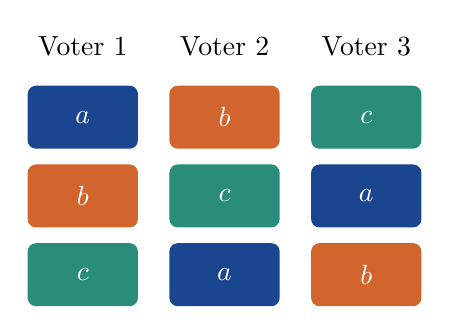
\begin{tikzpicture}[
        c/.style={rounded corners=3pt,minimum width=14mm,
          minimum height=8mm,text=white,font=\bfseries},
        a/.style={c,fill=tb},
        b/.style={c,fill=to},
        cc/.style={c,fill=tt}]
        \foreach \x/\v in {0/1,1.8/2,3.6/3}
          \node at (\x,0.9) {Voter \v};
        \node[a]  at (0,0)    {$a$};
        \node[b]  at (0,-1)   {$b$};
        \node[cc] at (0,-2)   {$c$};
        \node[b]  at (1.8,0)  {$b$};
        \node[cc] at (1.8,-1) {$c$};
        \node[a]  at (1.8,-2) {$a$};
        \node[cc] at (3.6,0)  {$c$};
        \node[a]  at (3.6,-1) {$a$};
        \node[b]  at (3.6,-2) {$b$};
      \end{tikzpicture}
    \end{column}
    \begin{column}{0.5\textwidth}
      \begin{itemize}
        \item<1-> Each voter ranks the candidates
        \item<2-> $a$ beats $b$, two voters to one
        \item<3-> $b$ beats $c$, two to one
        \item<4-> $c$ beats $a$, two to one
      \end{itemize}
    \end{column}
  \end{columns}
\end{frame}

\begin{frame}{The majority relation has a cycle}
  \begin{columns}
    \begin{column}{0.45\textwidth}
      \centering
      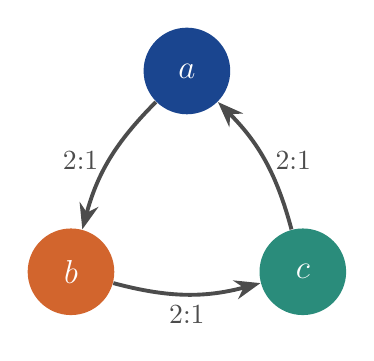
\begin{tikzpicture}[>=Stealth,
        v/.style={circle,minimum size=11mm,text=white,
          font=\large},
        every edge/.style={draw,->,line width=1.4pt,
          black!70}]
        \node[v,fill=tb] (a) at (90:1.7) {$a$};
        \node[v,fill=to] (b) at (210:1.7) {$b$};
        \node[v,fill=tt] (c) at (330:1.7) {$c$};
        \path (a) edge[bend right=15] node[left] {$2{:}1$} (b)
              (b) edge[bend right=15] node[below] {$2{:}1$} (c)
              (c) edge[bend right=15] node[right] {$2{:}1$} (a);
      \end{tikzpicture}
    \end{column}
    \begin{column}{0.55\textwidth}
      \begin{block}{Condorcet's paradox}
        Individual rankings are transitive. The majority relation need not be.
      \end{block}
      \begin{itemize}
        \item Every candidate loses to another one
        \item No \alert{Condorcet winner} exists
      \end{itemize}
    \end{column}
  \end{columns}
\end{frame}

\begin{frame}{A Condorcet winner beats every other candidate}
  \begin{columns}
    \begin{column}{0.45\textwidth}
      \centering
      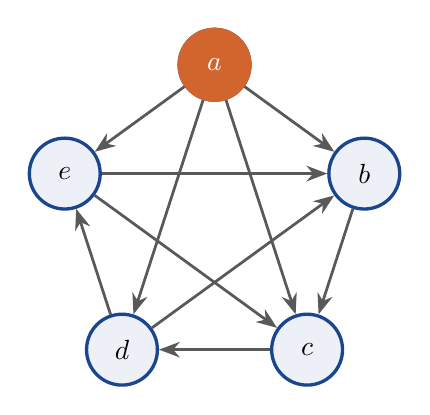
\begin{tikzpicture}[>=Stealth,
        v/.style={circle,draw=tb,line width=1.2pt,fill=tb!8,minimum size=9mm},
        every edge/.style={draw,->,line width=1pt,black!65}]
        \foreach \n [count=\i from 0] in {a,b,c,d,e}
          \node[v] (\n) at ({90-72*\i}:2) {$\n$};
        \node[v,fill=to,draw=to,text=white] at (a) {$a$};
        \path (a) edge (b) (a) edge (c) (a) edge (d) (a) edge (e)
              (b) edge (c) (c) edge (d) (d) edge (b)
              (e) edge (b) (e) edge (c) (d) edge (e);
      \end{tikzpicture}
    \end{column}
    \begin{column}{0.55\textwidth}
      \begin{itemize}
        \item An arrow $x \to y$: a majority prefers $x$ to $y$
        \item Here \alert{$a$} beats all four others
        \item Among $b,\dots,e$ the relation has cycles
      \end{itemize}
      \begin{block}{Condorcet consistency}
        A rule is Condorcet consistent if it elects the Condorcet winner whenever there is one.
      \end{block}
    \end{column}
  \end{columns}
\end{frame}

\begin{frame}{Borda and plurality can disagree}
  \begin{columns}
    \begin{column}{0.5\textwidth}
      \centering
      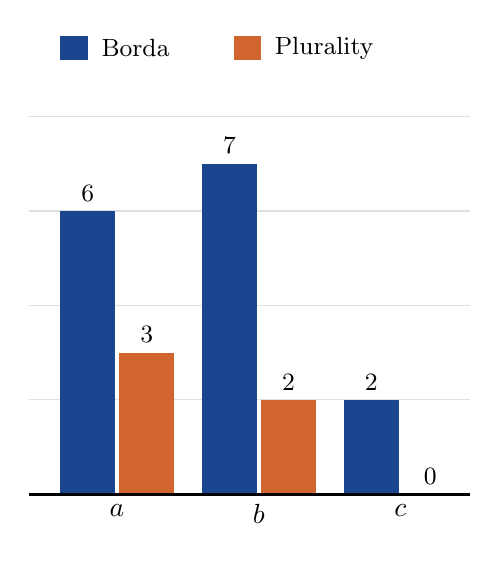
\begin{tikzpicture}[y=0.6cm]
        \foreach \y in {2,4,6,8} \draw[black!12] (0,\y) -- (5.6,\y);
        \foreach \x/\b/\p/\l in {0.4/6/3/a, 2.2/7/2/b, 4.0/2/0/c} {
          \fill[tb] (\x,0) rectangle +(0.7,\b);
          \fill[to] (\x+0.75,0) rectangle +(0.7,\p);
          \node[above,font=\small] at (\x+0.35,\b) {\b};
          \node[above,font=\small] at (\x+1.1,\p) {\p};
          \node[below] at (\x+0.72,0) {$\l$};
        }
        \draw[line width=0.8pt] (0,0) -- (5.6,0);
        \fill[tb] (0.4,9.2) rectangle +(0.35,0.5); \node[right,font=\small] at (0.8,9.45) {Borda};
        \fill[to] (2.6,9.2) rectangle +(0.35,0.5); \node[right,font=\small] at (3.0,9.45) {Plurality};
      \end{tikzpicture}
    \end{column}
    \begin{column}{0.5\textwidth}
      \begin{itemize}
        \item 3 voters: $a \succ b \succ c$
        \item 2 voters: $b \succ c \succ a$
        \item Borda gives $2,1,0$ points by position
      \end{itemize}
      \begin{exampleblock}{Result}
        Plurality elects $a$. Borda elects $b$.
      \end{exampleblock}
    \end{column}
  \end{columns}
\end{frame}

\begin{frame}{May's theorem}
  \begin{theorem}[May, 1952]
    For two candidates, majority rule is the only rule that is anonymous, neutral, and positively responsive.
  \end{theorem}
  \begin{proof}[Proof sketch]
    Anonymity and neutrality make the outcome depend only on the number of votes for each side. Positive responsiveness then fixes the threshold at one half.
  \end{proof}
\end{frame}

\end{document}
